\section{Appendix}

\subsection{Reachable set accuracy}
\label{subsec:appendix-reach-set-accuracy}
Suppose the track is defined in a stationary $(x, y)$ frame, $\theta$ is the vehicle's orientation and 
$\ell$ is the look ahead distance. 
%
As a part of experimentation, we perform the reachable set computation in Flow* and CORA by modeling a single turn on the track as the hybrid automata. 
%
The initial set is given as intervals over state variables i.e., $x \in [0.0, 0.5]$, $y \in [0.9, 1.1]$ and $\theta \in [-0.5, -0.5]$. 
%
The reachable sets computed in both tools are shown in figures~\ref{fig:reachSet1_flow} and ~\ref{fig:reachSet1_cora}. 
%
The divergent behavior of the reachable set in Flow* is seemingly due to error compounded over time because of coarse approximation. 
%
The figures also illustrate that the vehicle while turning swings to some extent before merging back on to the track.

\begin{figure*}
    \centering
    \subfigure[Flow*]{\label{fig:reachSet1_flow}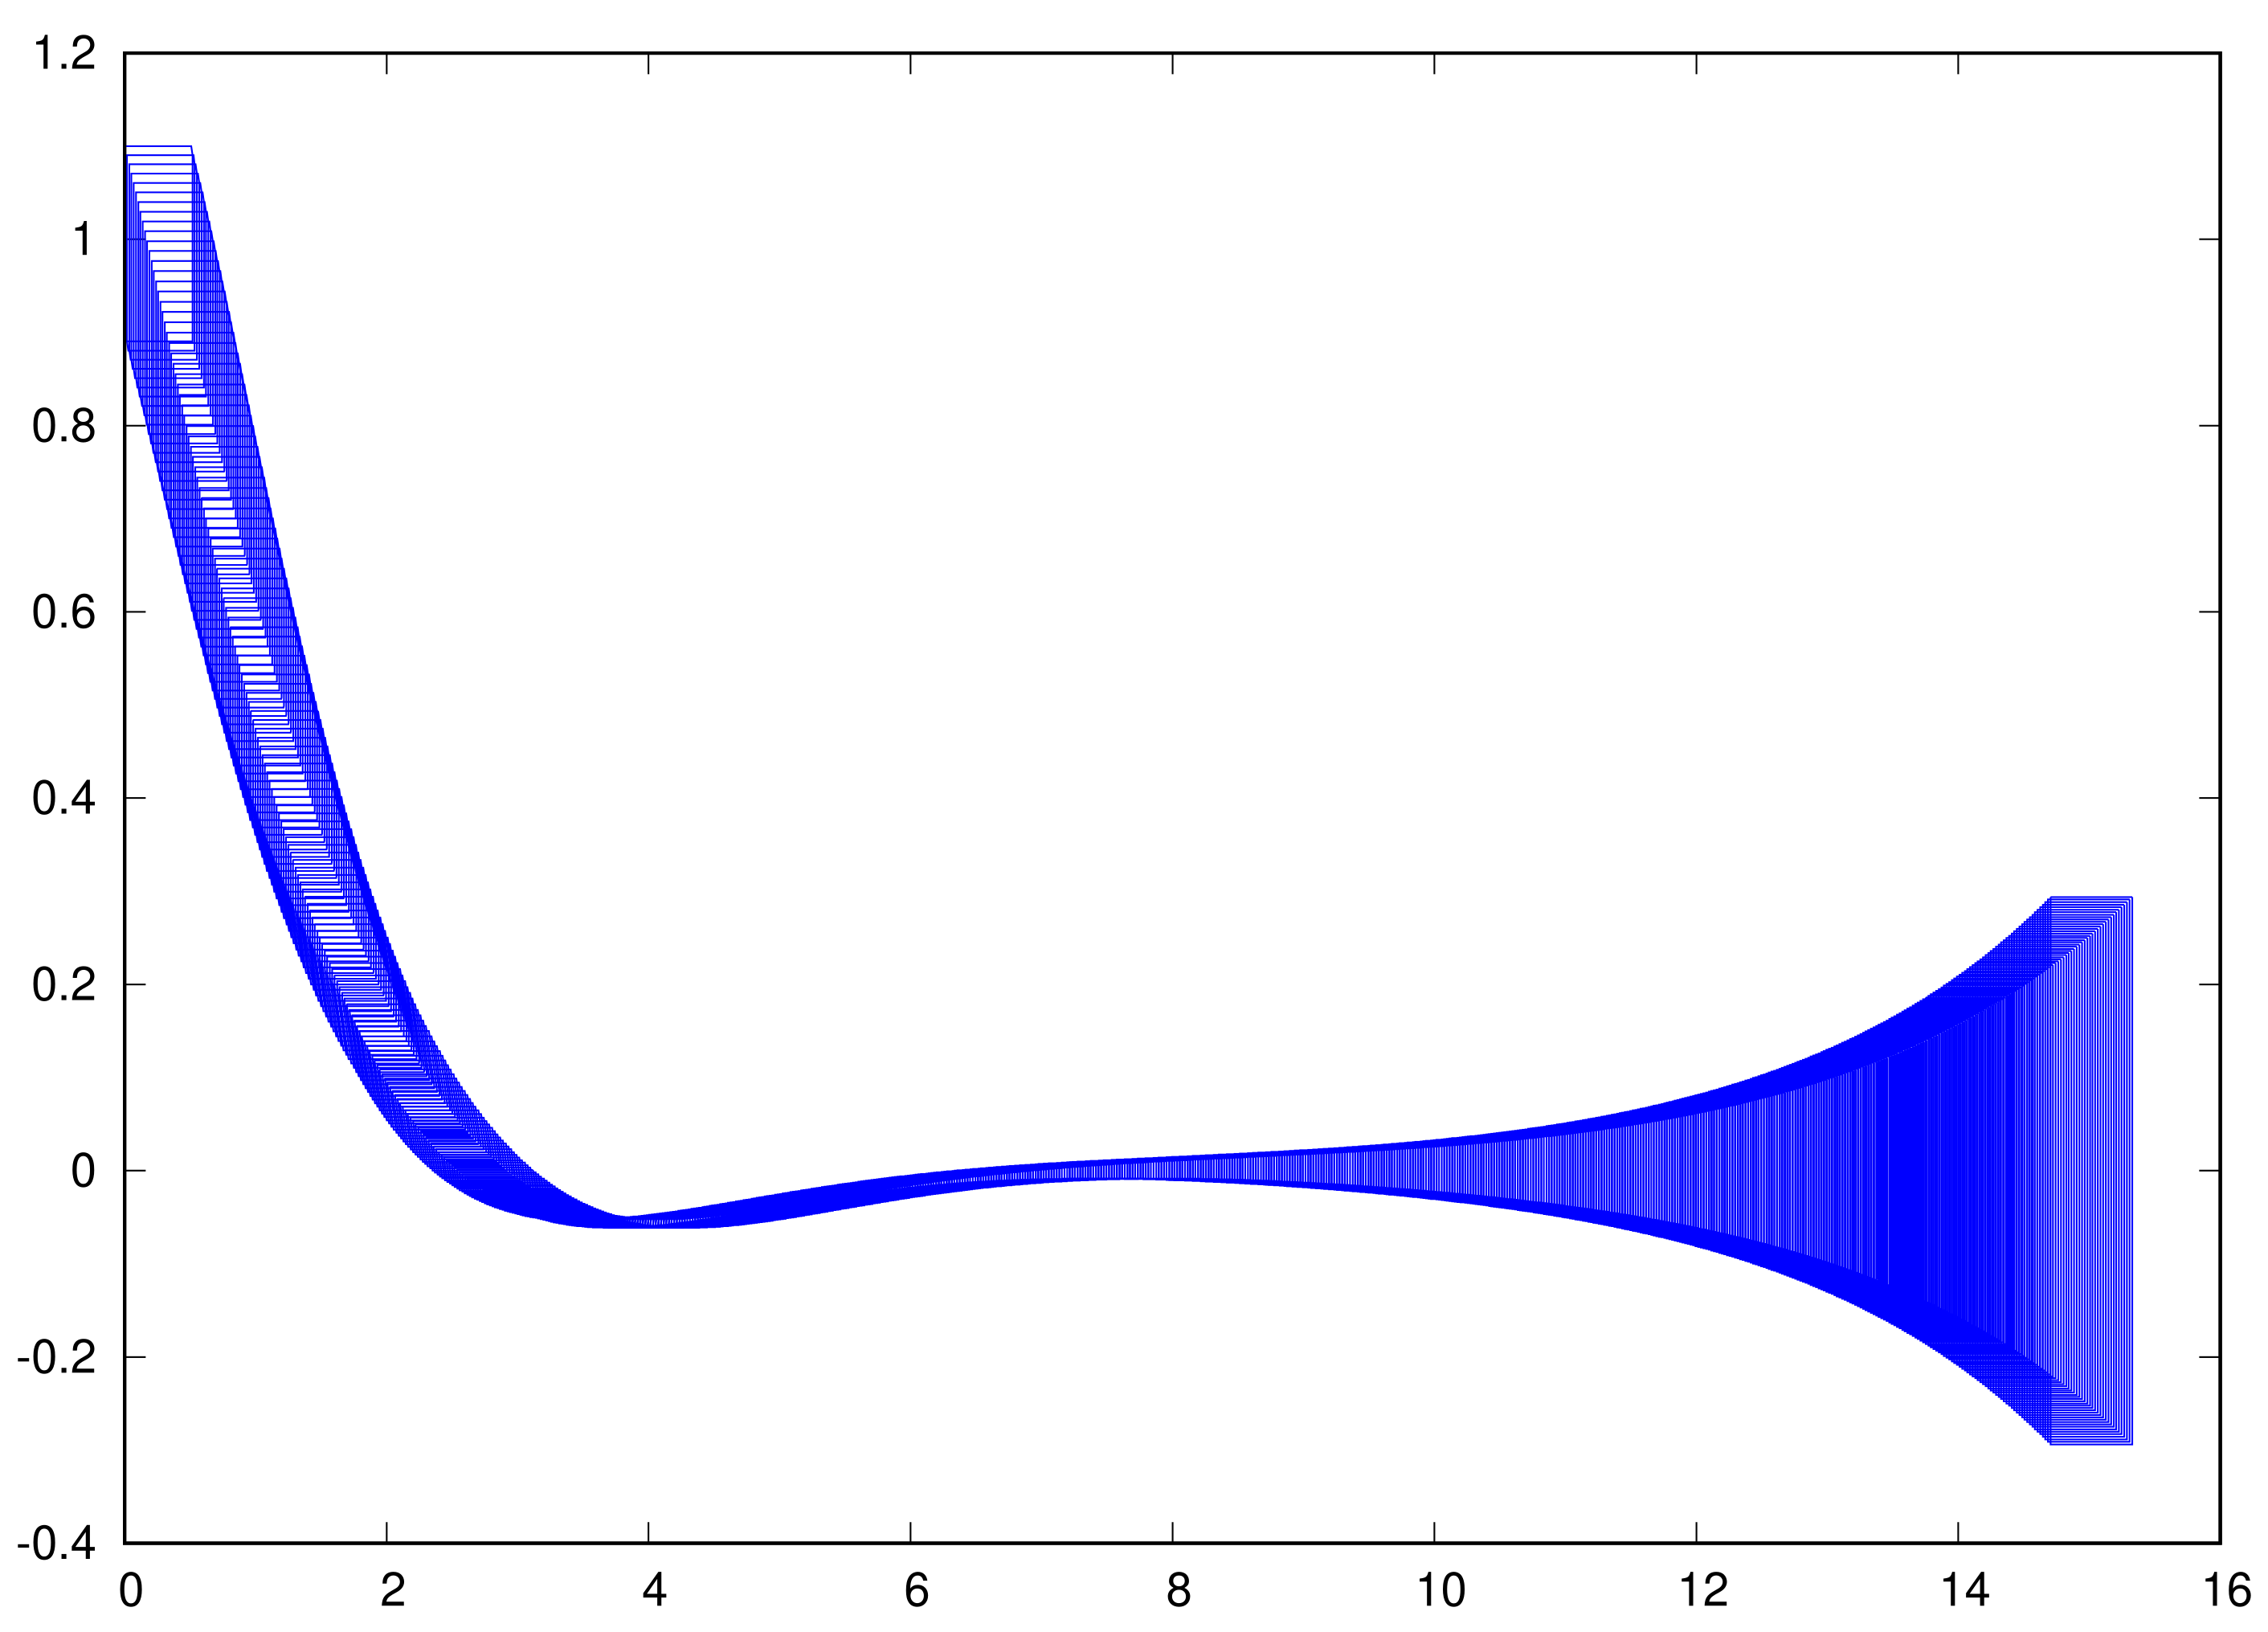
\includegraphics[width=87mm]{Figures/reachSet_1_flow_cropped.png}}
    \subfigure[CORA]{\label{fig:reachSet1_cora}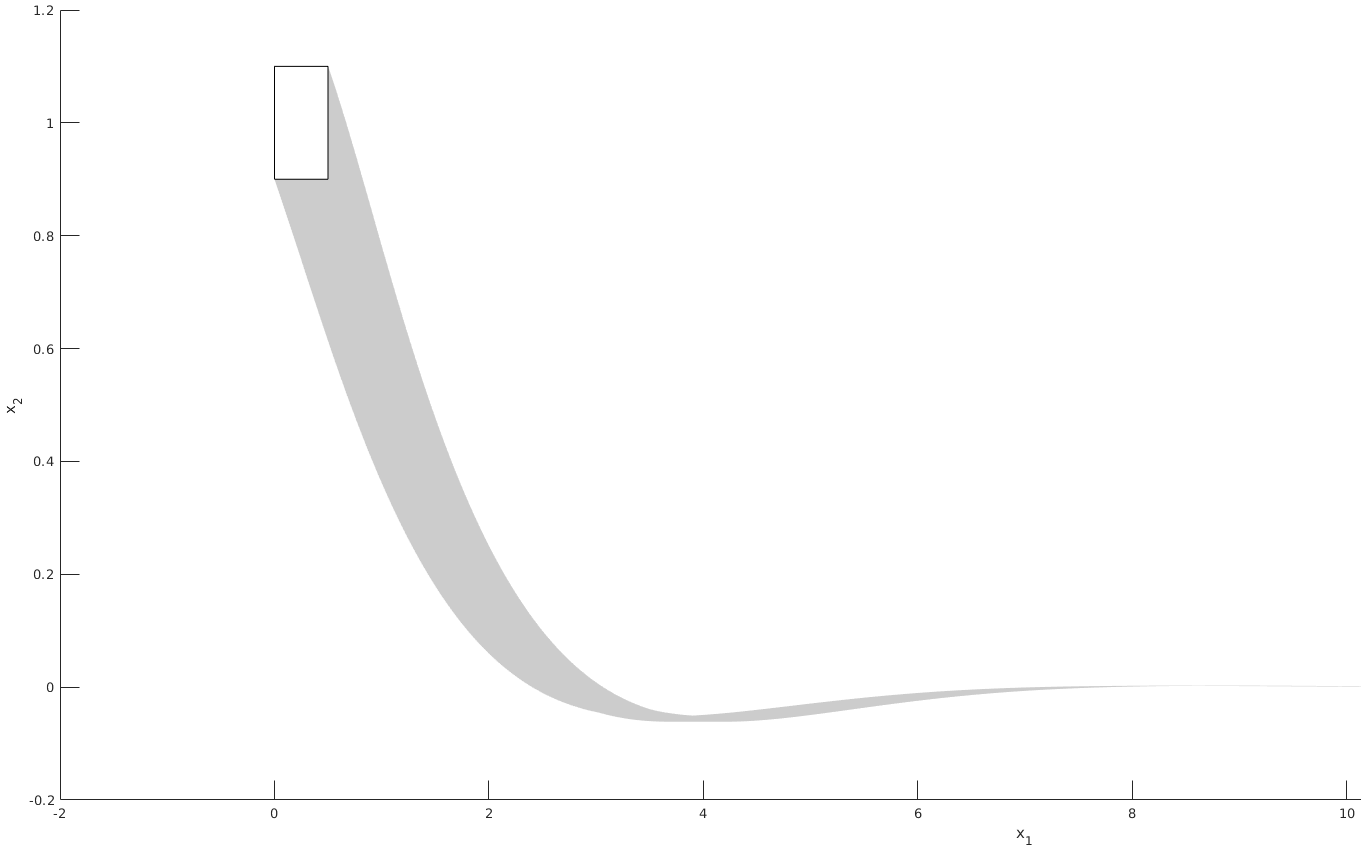
\includegraphics[width=87mm]{Figures/reachSet_1_cora_cropped.png}}
    \caption{Reachable sets computed in Flow* and CORA with time step 0.02 sec and time bound 15 sec for a set of initial states. The vehicle follows a vertical path downwards before making  a left turn.}
\label{fig:reachSets}
\end{figure*}

\begin{figure*}
    \centering
    \subfigure[Track 1-X]{\label{fig:track1-loc3-x}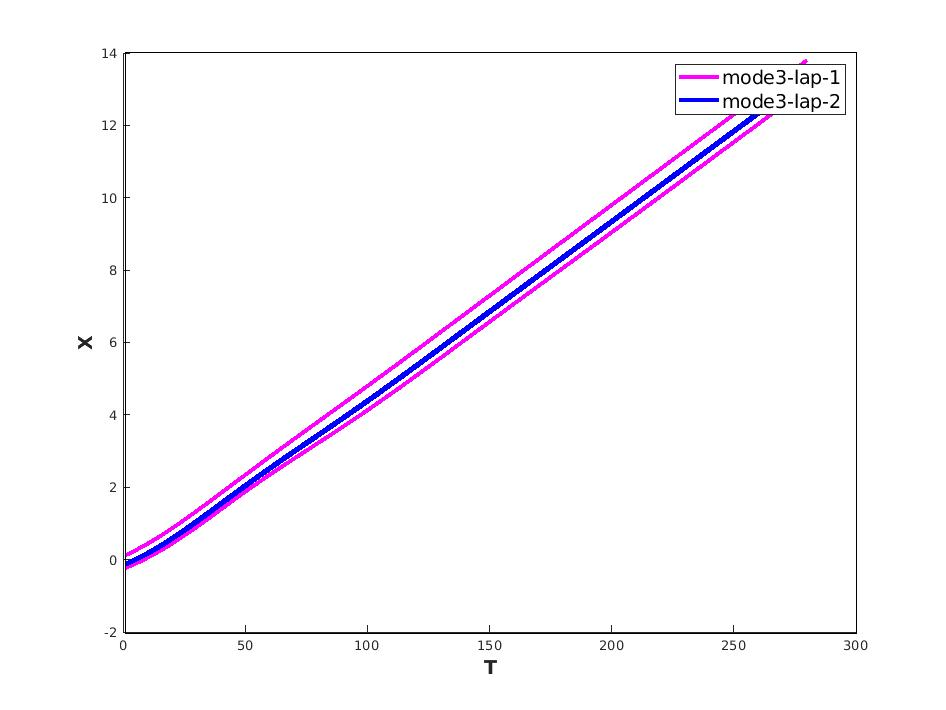
\includegraphics[width=87mm]{Figures/tracks/traci1-loc3-x.jpg}}
    \subfigure[Track 1-Y]{\label{fig:track1-loc3-y}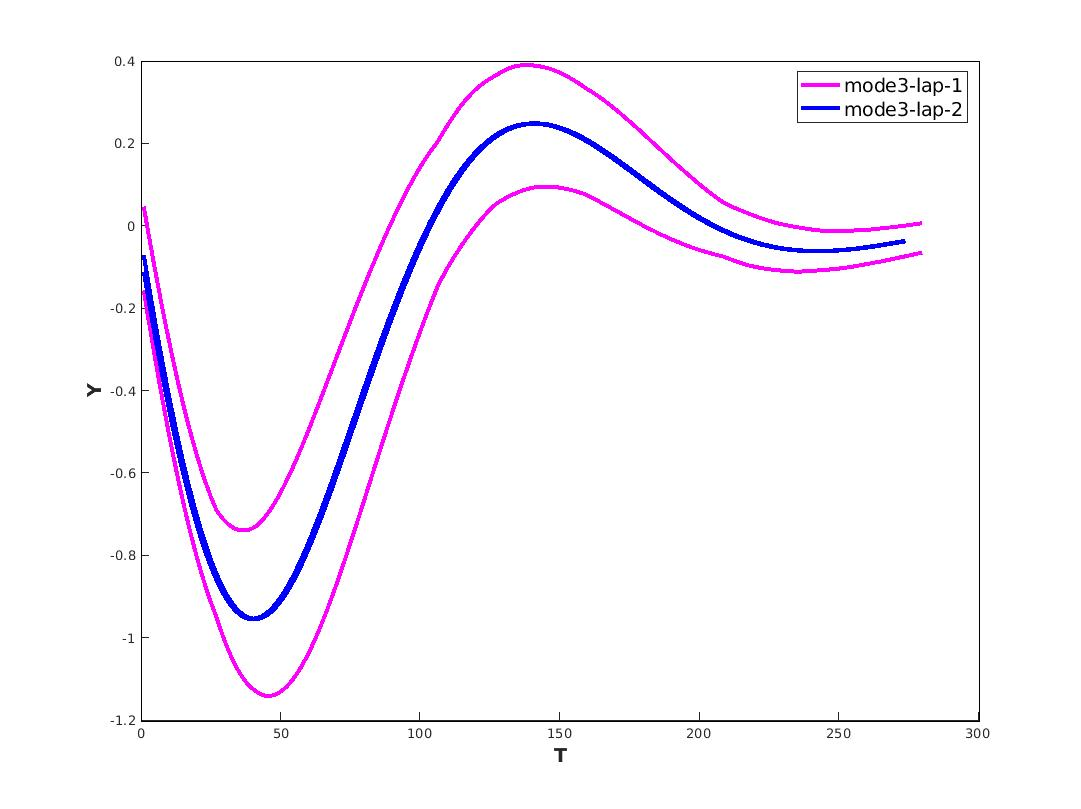
\includegraphics[width=87mm]{Figures/tracks/track1-loc3-y.jpg}}
    \subfigure[Track 1-$\theta$]{\label{fig:track1-loc3-theta}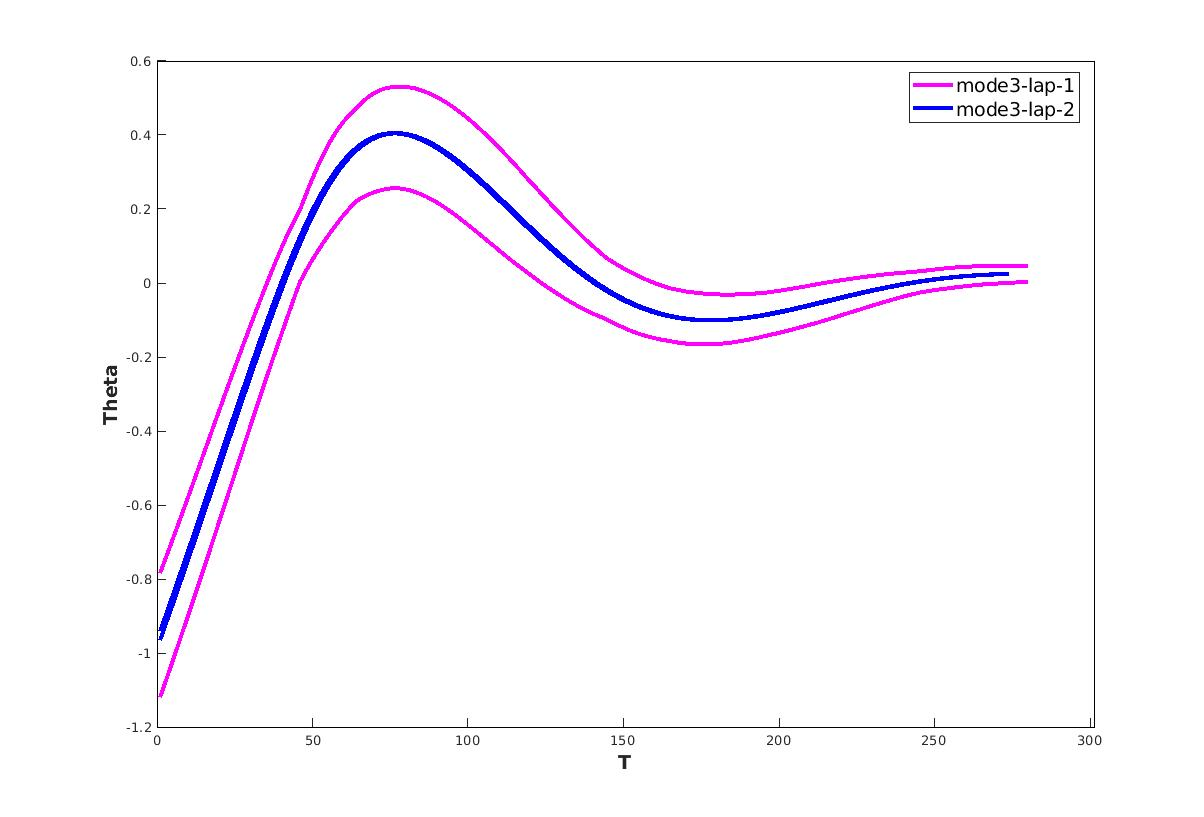
\includegraphics[width=87mmin]{Figures/tracks/track1-loc3-theta.jpg}}
    \caption{\textbf{Fixed point illustration using state variables in Track-1}}
\label{fig:track1-fixed-point-loc3}
\end{figure*}


\begin{figure*}
    \centering
    \subfigure[Track 2]{\label{fig:track2-voronoi-cora}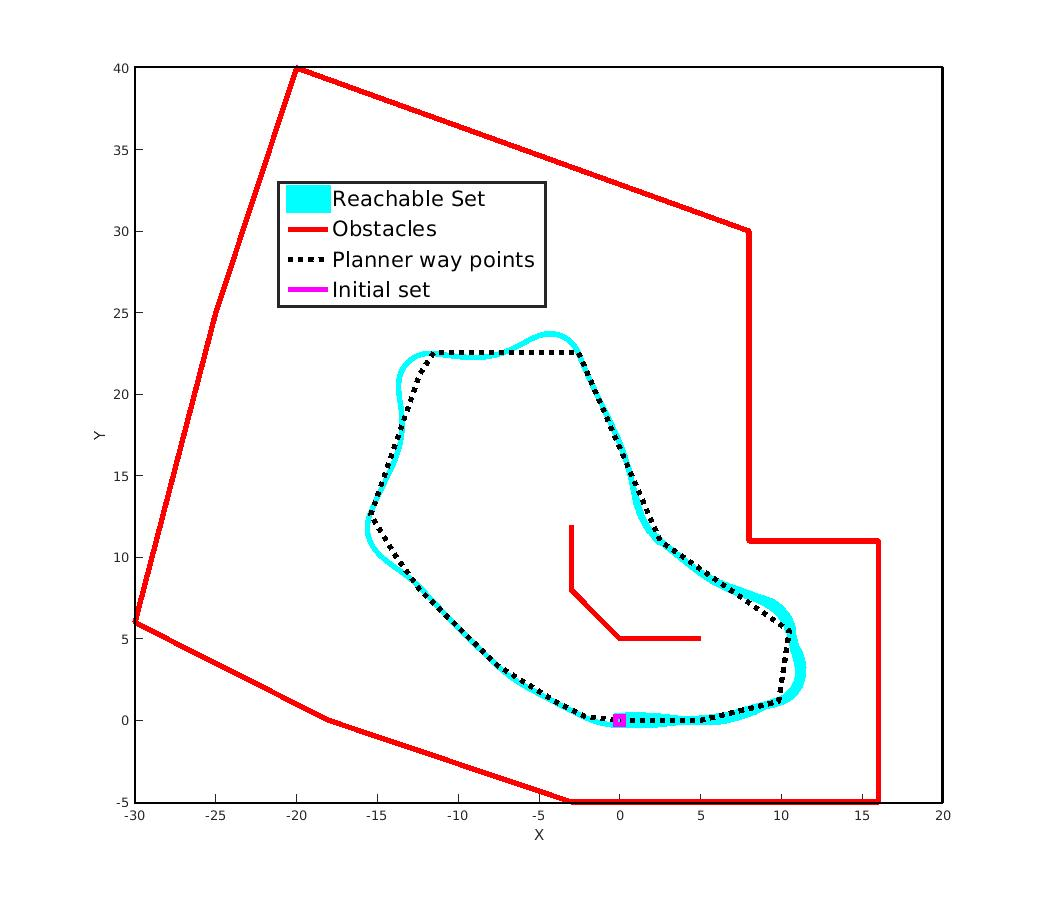
\includegraphics[width=87mm]{Figures/tracks/track2-voronoi-cora.jpg}}
    \subfigure[Track 3]{\label{fig:track3-voronoi-cora}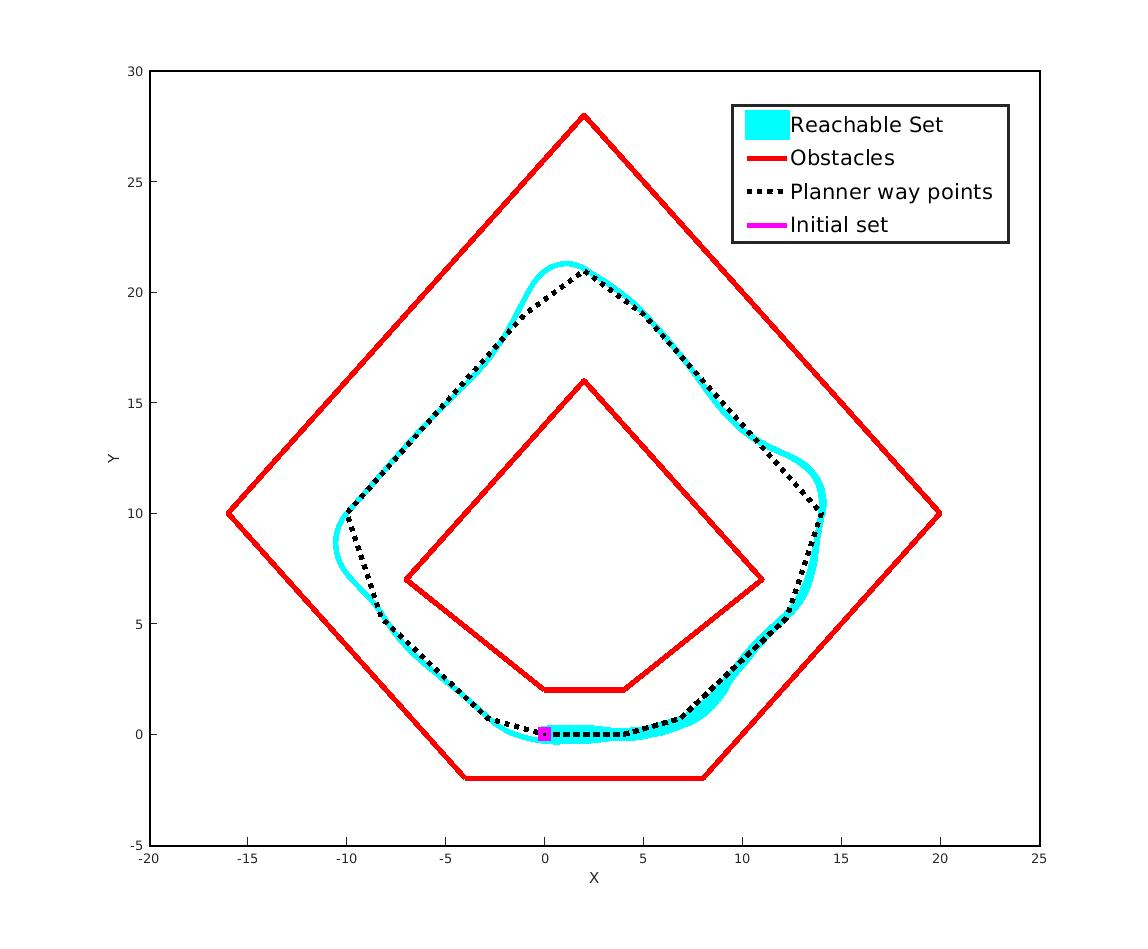
\includegraphics[width=87mm]{Figures/tracks/track3-voronoi-cora.jpg}}
    \subfigure[Track 4]{\label{fig:track4-voronoi-cora}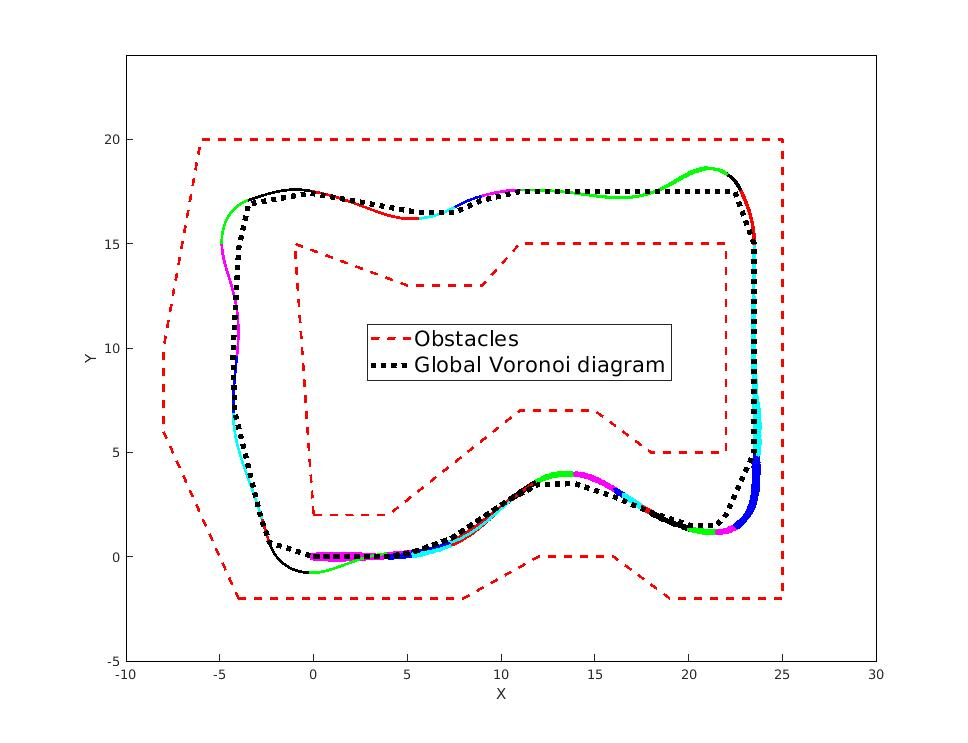
\includegraphics[width=87mm]{Figures/tracks/track4-voronoi-cora.jpg}}
    \subfigure[Track 5]{\label{fig:track5-voronoi-cora}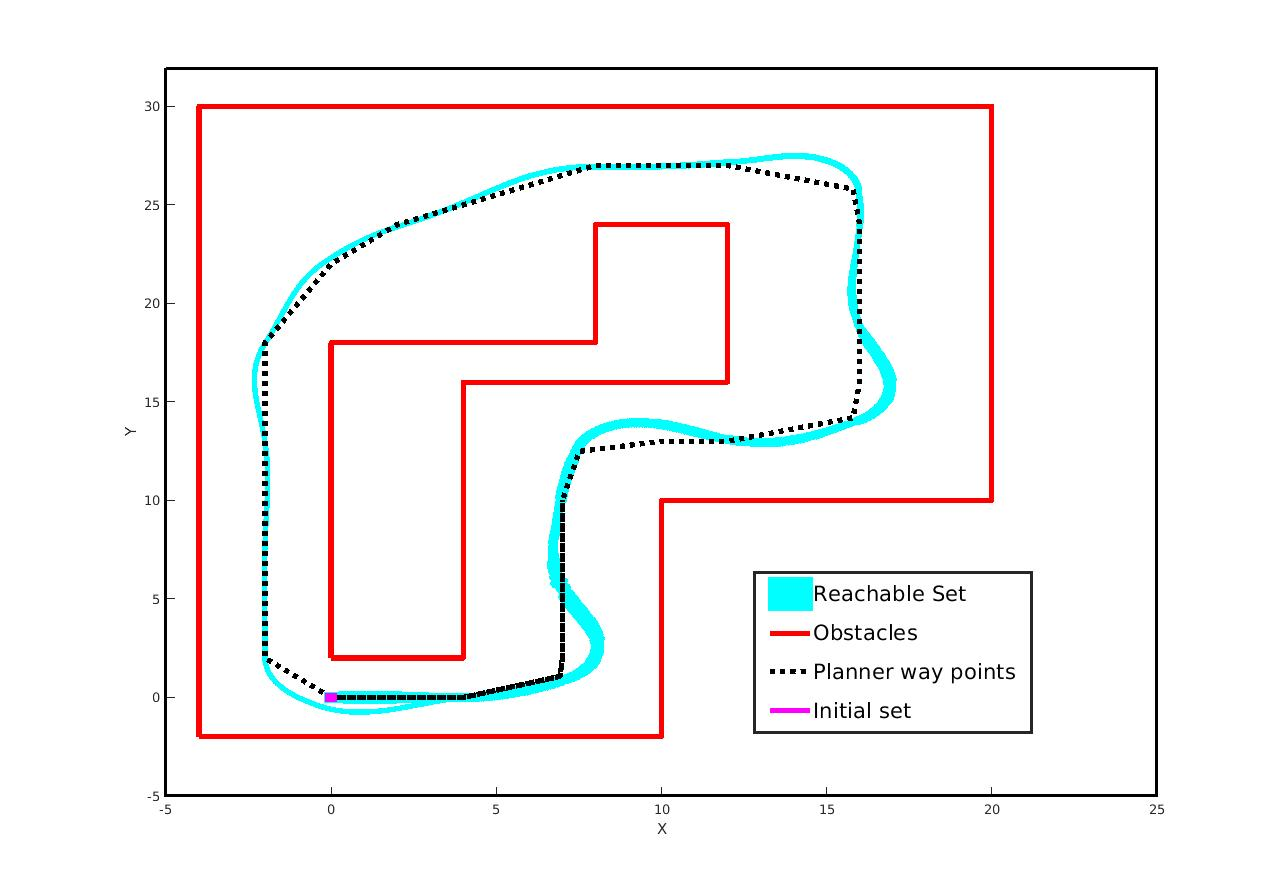
\includegraphics[width=87mm]{Figures/tracks/track5-voronoi-cora.jpg}}
    \caption{Safety verification of the plan in multiple other tracks. The track-wise initial sets are $\Theta_{2} = [[-0.25, 0.25][-0.25, 0.25][-0.15,0.15]]$, $\Theta_{3} = [[-0.2, 0.2][-0.2, 0.2][-0.2,0.2]]$, $\Theta_{4} = [[-0.12, 0.12][-0.12, 0.12][-0.12,0.12]]$, and $\Theta_{5} = [[-0.12, 0.12][-0.12, 0.12][-0.12,0.12]]$}
\label{fig:eval_track2-track3-track4-track5}
\end{figure*}
